本题将课程提供的 600 张图像划分为六个簇，考察不使用课程类别标签进行拟合时，图像表示能否反映语义类别。主方法预先固定为冻结 ResNet-18 特征、逐样本 $L_2$ 归一化及 K-means 聚类；以颜色纹理表示、PCA 降维和 Ward 凝聚聚类作为对照。方案及主结果随机种子均在读取外部评价分数之前固定，所有预定对照一并报告。

\IfFileExists{figures/method-overview.pdf}{%
\begin{figure*}[t]
\centering
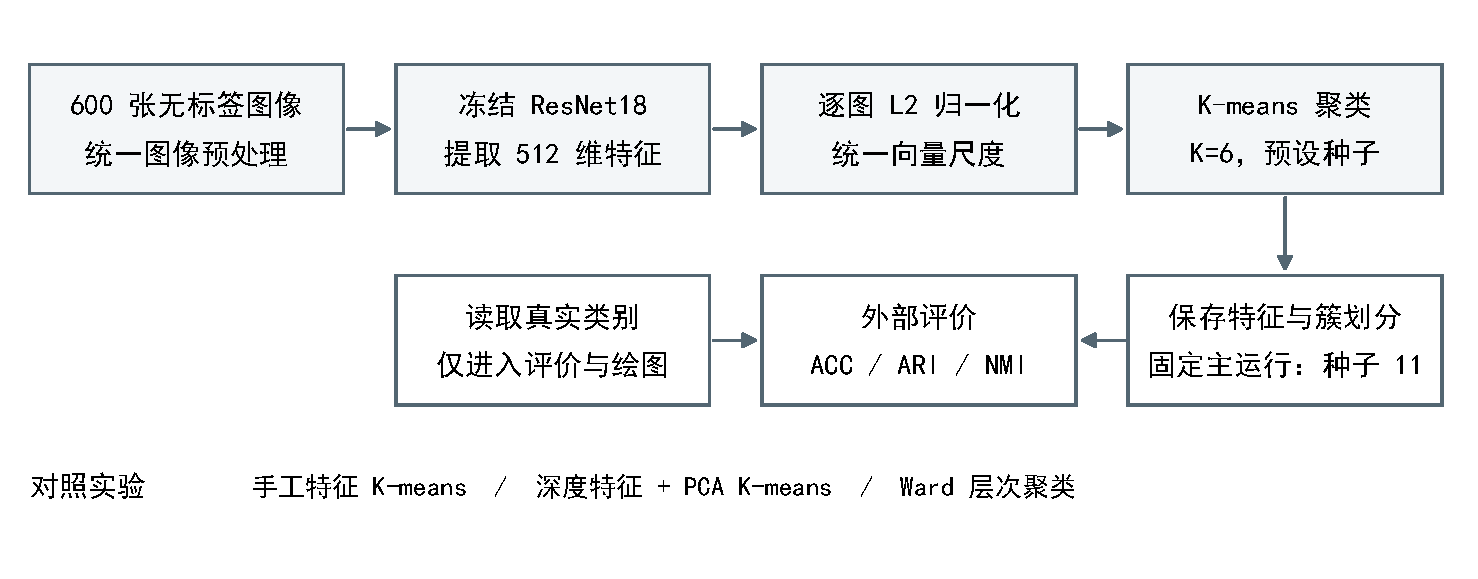
\includegraphics[width=0.96\textwidth]{figures/method-overview.pdf}
\Description{图像经固定的颜色纹理表示或冻结深度网络提取特征，完成归一化后进入 K-means 或 Ward 聚类；类别标签仅在聚类后参与外部评价。}
\caption{本轮实验程序的表示、聚类及评价流程。主方法采用冻结 ResNet-18 的 512 维归一化特征与 K-means。}
\label{fig:task1-overview}
\end{figure*}
}{}

\subsection{任务定义与信息使用范围}
记图像集合为 $\mathcal X=\{I_i\}_{i=1}^{N}$，其中 $N=600$。算法根据图像生成特征 $z_i\in\R^d$，输出簇编号 $c_i\in\{1,\ldots,K\}$，簇数按题目要求设为 $K=6$。初始数据核查涉及标签格式、类别数量及按类样例；类别标签 $y_i$ 不进入特征拟合、中心初始化、随机种子选择及模型选择。本轮实验程序先保存全部簇划分，再关联标签计算外部指标与绘图。簇编号没有预先给定的语义，不能将编号相等直接当作分类正确。

本实验在全部 600 张图像上提取特征并聚类，PCA 也只拟合这些图像的无标签特征。报告描述的是这批图像上的聚类结构，没有独立留出的新图像测试集。冻结网络的权重来自 ImageNet 有监督预训练，因此本文使用的是带有外部预训练知识的无监督聚类流程，不是从随机初始化出发的纯无监督视觉学习。

\subsection{颜色与局部纹理基线}
传统表示先将每张图像转为 RGB 并双线性缩放至 $224\times224$。通过 Pillow 转换为 HSV，将通道整数值除以 256 后放入 $[0,1]$ 的分箱范围，使用 $8\times4\times4$ 个分箱构造联合直方图 $h_i^{\mathrm{HSV}}\in\R^{128}$。直方图刻画整幅图像的颜色组成，不显式编码物体位置和轮廓。

纹理分支将图像转换为 uint8 灰度图，计算邻域点数 $P=8$、半径 $R=1$ 的 uniform LBP\citep{ojala2002}。该描述将局部邻域与中心像素比较，统计环形二进制模式；uniform 模式按正比较的个数编码，非 uniform 模式归为一类，得到 $P+2=10$ 维直方图 $h_i^{\mathrm{LBP}}$。它表征局部亮度变化模式，不能单独保证语义类别可分。

对两个直方图分别作 $L_1$ 归一化后逐元素开平方：
\begin{equation}
q_i^{(b)}=\sqrt{\frac{h_i^{(b)}}{\|h_i^{(b)}\|_1}},
\qquad b\in\{\mathrm{HSV},\mathrm{LBP}\}.
\end{equation}
非空图像的两个直方图均具有正总计数。拼接后再作 $L_2$ 归一化，得到 138 维颜色纹理表示：
\begin{equation}
z_i^{\mathrm{hand}}=
\frac{[q_i^{\mathrm{HSV}};q_i^{\mathrm{LBP}}]}
{\|[q_i^{\mathrm{HSV}};q_i^{\mathrm{LBP}}]\|_2}.
\end{equation}
平方根变换对应直方图的 Hellinger 表示。每个分支变换后的平方范数均为 1，因此拼接时两个分支具有相等总权重，避免颜色分箱数较多就自动占据更大的权重。

\subsection{冻结 ResNet-18 的全局表示}
深度分支采用 ResNet-18\citep{he2016resnet}，明确加载 Torchvision 的 \texttt{IMAGENET1K\_V1} 权重，冻结全部参数并切换至推理模式。使用该权重规定的预处理：按短边 256 缩放、中心裁剪为 $224\times224$，将 RGB 像素缩放至 $[0,1]$，再按通道均值 $(0.485,0.456,0.406)$ 和标准差 $(0.229,0.224,0.225)$ 标准化\citep{torchvisionresnet18}。这里采用确定性中心裁剪，没有随机增强或使用课程标签微调。

移除最终分类层，保留全局平均池化输出，得到
\begin{equation}
f_i=f_{\theta}^{\mathrm{avgpool}}(I_i)\in\R^{512},
\qquad
z_i=\frac{f_i}{\|f_i\|_2}.
\label{eq:deep-feature}
\end{equation}
其中 $\theta$ 为冻结参数。归一化前将特征转换为 float64，并检查向量非零且各元素有限；不合格时程序报错而非继续聚类。归一化使距离比较更多反映特征方向；对于两个单位向量，$\|z_i-z_j\|_2^2=2-2z_i^\top z_j$。这一等价关系针对样本之间的距离，不意味着普通 K-means 的中心也始终具有单位范数。

PCA 对照在上述 512 维归一化特征上拟合中心化 PCA，使用完整 SVD、保留 64 个主成分且不白化：
\begin{equation}
u_i=W_{64}^{\top}(z_i-\bar z),\qquad
z_i^{\mathrm{PCA}}=\frac{u_i}{\|u_i\|_2}.
\end{equation}
PCA 仅依据样本协方差压缩特征，随后再次 $L_2$ 归一化。该对照检验去除低方差方向是否影响聚类；高方差方向不必然等于最有语义区分力的方向，因此不预设降维一定改善结果。

\subsection{K-means 与 Ward 聚类}
K-means 以簇内平方距离和为目标：
\begin{equation}
\min_{\{c_i\},\{\mu_k\}}\ J
=\sum_{i=1}^{N}\|z_i-\mu_{c_i}\|_2^2.
\label{eq:kmeans}
\end{equation}
采用 Lloyd 交替更新\citep{lloyd1982}：将样本分配给最近中心，再把中心更新为所属样本均值。初始化使用 k-means++\citep{arthur2007}，每个随机种子执行 20 次初始化，每次最多迭代 300 轮，收敛容差为 $10^{-4}$，并按最小目标函数值保留该种子的一次结果。这一内部选择依据无标签目标函数，不依据 ACC、ARI 或 NMI。

每种 K-means 方案使用五个固定种子：11、23、37、53 和 71。主结果采用种子 11，其余种子用于均值、标准差与稳定性分析，不从五个种子中挑选外部指标最高的一次。

Ward 对照使用与主方法相同的 512 维归一化深度特征，从单样本簇开始逐步合并，每次选择导致簇内平方和增加最少的两个簇\citep{ward1963}。两簇 $A,B$ 的合并代价为
\begin{equation}
\Delta(A,B)=\frac{|A||B|}{|A|+|B|}
\|\mu_A-\mu_B\|_2^2.
\end{equation}
合并至六簇停止。固定输入顺序下该实现不使用随机初始化，因而只报告一次结果，不把重复相同运行解释为随机稳定性证据。
